\section{Diseño}
\begin{frame}{Circuitos equivalentes}
  \begin{minipage}[t]{0.45\textwidth}
    \resizebox{\textwidth}{!}{
      \begin{tikzpicture}
      % Paths, nodes and wires:
      \node[npn, rotate=90, yscale=-1](N1) at (0, -0){} node[anchor=south] at (N1.text){$Q_1$};
      \draw (-0.77, 0) |- (-3, -0);
      \draw (0.77, -0) -- (3, -0);
      \draw (-3, -0.84) to[american resistor, l={$R_E$}] (-3, -2.75);
      \draw (3, -0.84) to[american resistor, l={$R_C$}] (3, -2.75);
      \draw (-3, -0.84) -| (-3, -0);
      \draw (3, -0) -| (3, -0.84);
      \node[vcc](N2) at (5, -3){} node[anchor=south] at (N2.text){$V_{CC}$};
      \draw (5, -3) -| (5, -4) -- (3, -4);
      \draw (-3, -2.75) |- (-3, -4);
      \draw (3, -2.75) -| (3, -4);
      \node[ground] at (-3, -4){};
      \draw (-3, -0) -- (-4, -0);
      \draw (3, -0) -- (6, -0);
      \node[ocirc](N3) at (-4, -0){} node[anchor=east] at (N3.text){$V_i$};
      \node[ocirc](N4) at (6, -0){} node[anchor=west] at (N4.text){$V_o$};
      \draw (-2.41, -3.5) to[american resistor, l={$R_1$}] (-0.5, -3.5);
      \draw (0.5, -3.5) to[american resistor, l={$R_2$}] (2.41, -3.5);
      \draw (-2.41, -3.5) -- (-3, -3.5);
      \draw (-0.5, -3.5) -- (0.5, -3.5);
      \draw (2.41, -3.5) -- (3, -3.5);
      \draw (0, -3.5) |- (-0, -0.84);
    \end{tikzpicture}
    }
    Según (Ec. \ref{eq:r1}) y (Ec. \ref{eq:r2}) tenemos que:
    \begin{equation*}
      R_1 = \frac{R_B}{1 - \frac{V_{BB}}{V_{CC}}} \quad R_2 = \frac{V_{CC} R_B}{V_{BB}}
    \end{equation*}
  \end{minipage}
  \begin{minipage}{0.08\textwidth}
    \begin{equation*}
      \equiv
    \end{equation*}
  \end{minipage}
  \begin{minipage}[t]{0.45\textwidth}
    \resizebox{\textwidth}{!}{
    \begin{tikzpicture}
      % Paths, nodes and wires:
      \node[npn, rotate=90, yscale=-1](N1) at (0, -0){} node[anchor=south] at (N1.text){$Q_1$};
      \draw (-0, -0.84) to[american resistor, l={$R_B$}] (0, -2.75);
      \draw (-0.77, 0) |- (-3, -0);
      \draw (0.77, -0) -- (3, -0);
      \draw (-3, -0.84) to[american resistor, l={$R_E$}] (-3, -2.75);
      \draw (3, -0.84) to[american resistor, l={$R_C$}] (3, -2.75);
      \draw (0, -2.75) to[battery, l={$V_{BB}$}] (0, -4);
      \draw (-3, -0.84) -| (-3, -0);
      \draw (3, -0) -| (3, -0.84);
      \node[vcc](N2) at (5, -3){} node[anchor=south] at (N2.text){$V_{CC}$};
      \draw (5, -3) -| (5, -4) -- (3, -4);
      \draw (-3, -2.75) |- (0, -4);
      \draw (3, -2.75) -| (3, -4);
      \node[ground] at (0, -4){};
      \draw (-3, -0) -- (-4, -0);
      \draw (3, -0) -- (6, -0);
      \node[ocirc](N3) at (-4, -0){} node[anchor=east] at (N3.text){$V_i$};
      \node[ocirc](N4) at (6, -0){} node[anchor=west] at (N4.text){$V_o$};
    \end{tikzpicture}
    }
    Según (Ec. \ref{ec:thevenin-rb}) y (Ec. \ref{ec:thevenin-vbb}) tenemos que:
    \begin{equation*}
      R_B = \frac{R_1 R_2}{R_1 + R_2} \quad V_{BB} = \frac{V_{CC} R_1}{R_1 + R_2}
    \end{equation*}
  \end{minipage}
\end{frame}
\subsection{Punto Q}
\begin{frame}[allowframebreaks]{Polarización en CC}
  \begin{minipage}{0.3\textwidth}
    \resizebox{\textwidth}{!}{
    \begin{tikzpicture}
      % Paths, nodes and wires:
      \node[npn](N1) at (0, 0){} node[anchor=west] at (N1.text){$Q1$};
      \draw (0, -0.77) to[american resistor, l={$R_E$}] (0, -3);
      \draw (0, 3.02) to[american resistor, l={$R_C$}] (0, 0.77);
      \draw (0, -3) -| (0, -3.25);
      \node[vcc](N2) at (0, 3.02){} node[anchor=south] at (N2.text){$V_{cc}$};
      \node[ground] at (0, -3.75){};
      \draw (0, -3.25) -| (0, -3.75);
      \draw (-3.25, 0) to[american resistor, l={$R_B$}] (-3.25, -2.25);
      \draw (-3.25, 0) -- (-0.84, 0);
      \draw (-3.25, -3.5) -| (-3.25, -3.75) -- (0, -3.75);
      \draw (-3.25, -2.25) to[battery, l={$V_{BB}$}] (-3.25, -3.5);
      \draw (0, 0.77) -- (1, 0.77);
      \draw (0, -0.77) -- (1, -0.77);
      \node[ocirc](N3) at (1, -0.77){} node[anchor=west] at (N3.text){$V_i$};
      \node[ocirc](N4) at (1, 0.77){} node[anchor=west] at (N4.text){$V_o$};
    \end{tikzpicture}
    }
    \begin{align*}
      V_{CC} &= 15.2V \quad R_E = 220\Omega\\
      R_C &= 2K2\Omega \quad \beta = 484\\
      &\quad \quad R_L = 2K2\Omega
    \end{align*}
  \end{minipage}
  \begin{minipage}{0.6\textwidth}
    Aplicando el criterio de diseño:
    \begin{equation}
      R_B = R_E \frac{\beta}{10}
    \end{equation}
    Se obtiene:
    \begin{align*}
      R_B &= 2K2\Omega \frac{484}{10}\\[6pt]
      R_B &= 10648 \Omega
    \end{align*}
  \end{minipage}
  \begin{minipage}[][\textheight][]{\textwidth}
    Usando (Ec. \ref{ec:vbb}):
    \small
    \begin{align*}
      V_{BB} &= \frac{V_{CC} \left(R_E + \frac{R_B}{\beta}\right) + V_{BE} \left(R_C - \frac{R_B}{\beta} + R_C // R_L \right)}{R_E + R_C + R_C // R_L}\\[6pt]
      V_{BB} &= \frac{15.2V \left(220\Omega + \frac{10684\Omega}{484}\right) + 0.7V \left(2K2\Omega - \frac{10684\Omega}{484} + 2K2\Omega // 2K2\Omega \right)}{220\Omega + 2K2\Omega + 2K2\Omega // 2K2\Omega}\\[6pt]
      V_{BB} &= 1.69V
    \end{align*}
  \end{minipage}

  Procedemos a calcular $R_1$ y $R_2$ usando (Ec. \ref{eq:r1}) y (Ec. \ref{eq:r2}):
  \begin{figure}[!ht]
    \begin{minipage}{0.45\textwidth}
      \begin{align*}
        R_2 &= \frac{V_{CC} R_B}{V_{BB}}\\[6pt]
        R_2 &= \frac{15.2V \cdot 10648\Omega}{1.69V}\\[6pt]
        R_2 &= 95768.99\Omega
      \end{align*}
    \end{minipage}
    \hfill
    \begin{minipage}{0.45\textwidth}
      \begin{align*}
        R_1 &= \frac{R_B R_2}{R_2 - R_B}\\[6pt]
        R_1 &= \frac{95768.99\Omega \cdot 10648\Omega}{95768.99\Omega - 10648\Omega}\\[6pt]
        R_1 &= 11979.98\Omega
      \end{align*}
    \end{minipage}
  \end{figure}
  \begin{figure}[!ht]
    Por ultimo, calculamos $I_{CQ_{MES}}$ y $V_{CBQ_{MES}}$ usando (Ec. \ref{ec:iq-mes}) y (Ec. \ref{ec:vcb-mes}):
    \small
    \begin{minipage}{0.45\textwidth}
      \begin{align*}
        I_{CQ_{MES}} &= \frac{V_{CC} - V_{BB}}{R_C - \frac{R_B}{\beta} + R_C // R_L}\\[6pt]
        I_{CQ_{MES}} &= \frac{15.2V - 1.69V}{2K2\Omega - \frac{10648\Omega}{484} + 2K2\Omega // 2K2\Omega}\\[6pt]
        I_{CQ_{MES}} &= 4.121mA
      \end{align*}
    \end{minipage}
    \hfill
    \begin{minipage}{0.45\textwidth}
      \begin{align*}
        V_{CBQ_{MES}} &= V_{CC} - V_{BB} - I_{CQ_{MES}} \left(R_C - \frac{R_B}{\beta}\right)\\[6pt]
        V_{CBQ_{MES}} &= 15.2V - 1.69V - 4.121mA \left(2K2\Omega - \frac{10648\Omega}{484}\right)\\[6pt]
        V_{CBQ_{MES}} &= 4.53V
      \end{align*}
    \end{minipage}
  \end{figure}
\end{frame}

\begin{frame}[allowframebreaks]{Rectas de Carga}
  \begin{figure}[!h]
    \begin{minipage}[t]{0.45\textwidth}
      Recta de carga en CC:
      \begin{equation*}
        v_{CBQ} = V_{CC} - V_{BB} - i_C \left(R_C - \frac{R_B}{\beta}\right)
      \end{equation*}
    \end{minipage}
    \hfill
    \begin{minipage}[t]{0.45\textwidth}
      Recta de carga en CA:
      \begin{align*}
        v_{CB} &= V_{CC}' - i_C \frac{R_C R_L}{R_C + R_L}\\[6pt]
        V_{CC}' &= V_{CBQ_{MES}} + I_{CQ_{MES}}(R_C // R_L)
      \end{align*}
    \end{minipage}
  \end{figure}
  Los cortes en los ejes están dados por:
  \begin{figure}[!ht]
    \begin{minipage}{0.45\textwidth}
      Para CC:
      \small
      \begin{align*}
        &i_C \to 0, \quad v_{CB_{max}} = V_{CC} - V_{BB}\\[6pt]
        &v_{CB} \to 0, \quad i_{C_{max}} = \frac{V_{CC} - V_{BB}}{R_C - \frac{R_B}{\beta}}
      \end{align*}
    \end{minipage}
    \hfill
    \begin{minipage}{0.45\textwidth}
      Para CA:
      \small
      \begin{align*}
        &i_C \to 0, \quad v_{CB_{max}} = V_{CC}'\\[6pt]
        &v_{CB} \to 0, \quad i_{C_{max}} = \frac{V_{CBQ_{MES}}}{R_C // R_L} + I_{CQ_{MES}}
      \end{align*}
    \end{minipage}
  \end{figure}

  \begin{figure}[!h]
    \centering
    \begin{minipage}{0.45\textwidth}
      \centering
      \begin{tikzpicture}
        \begin{axis}[
            axis lines=middle,
            xlabel={$V_{CB}$ [V]},
            ylabel={$I_C$ [mA]},
            xmin=0, xmax=16,
            ymin=0, ymax=10,
            grid=both,
            width=6cm,
            height=6cm,
            xtick={0,2,...,15},
            ytick={0,2,...,7},
            legend style={fill=darkbg, draw=white},
        ]
          \addplot[red, thick] coordinates {(0,6.2) (13.51,0)};
          \addlegendentry{Recta CC}
          \addplot[blue, thick] coordinates {(0,8.23) (9.06,0)};
          \addlegendentry{Recta CA}
          \addplot[only marks, mark=*] coordinates {(4.525,4.125)};
          \node[above right] at (axis cs:4.525,4.125) {Q};
        \end{axis}
      \end{tikzpicture}
    \end{minipage}
    \hfill
    \begin{minipage}{0.45\textwidth}
      \begin{gather*}
        v_{CBQ_{CC}} = v_{CB_{CA}}\\[6pt]
        i_C = \frac{V_{CC} - V_{BB} - V_{CC}'}{R_C - \frac{R_B}{\beta} - R_C // R_L}\\[6pt]
        i_C = 4.125mA \to v_{CBQ} = 4.525V
      \end{gather*}
    \end{minipage}
    \caption{rectas de carga y punto Q extraído de las intersecciones de las rectas.}
  \end{figure}

\end{frame}

\begin{frame}{Simulación}
  \begin{figure}[!ht]
    \centering
    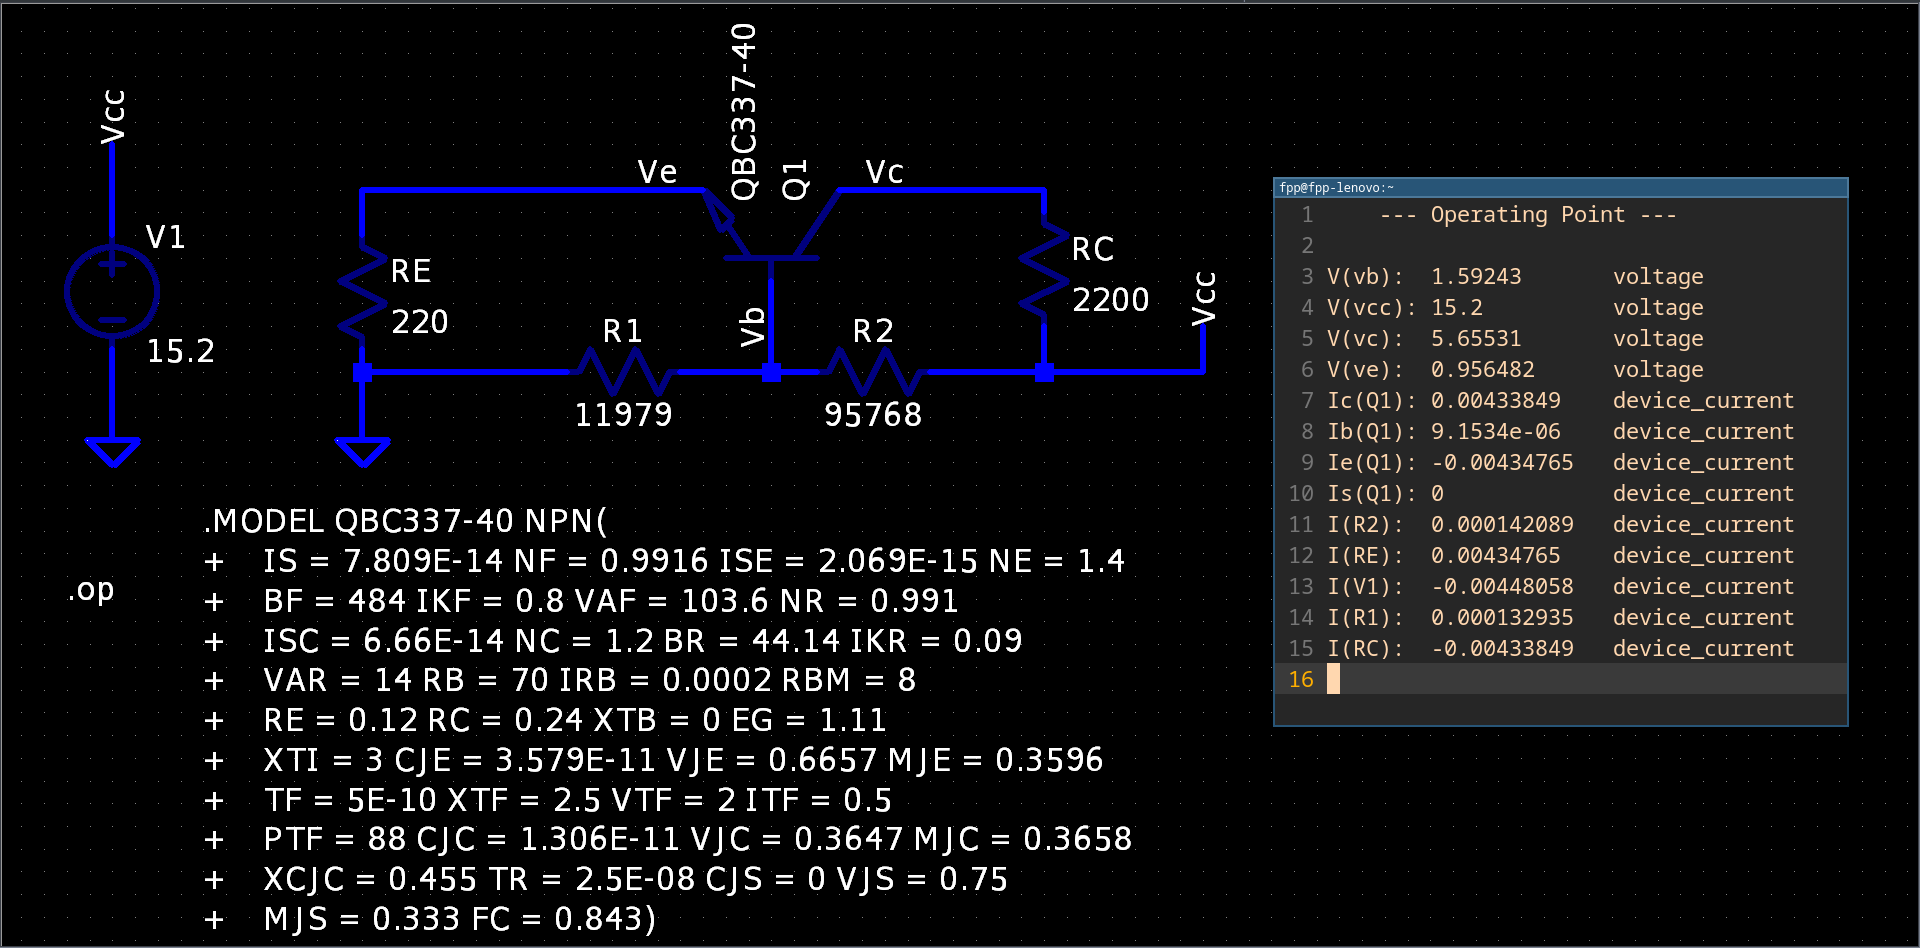
\includegraphics[width=.9\textwidth]{images/sim_calculada.png}
    \caption{simulación en LTSpice de punto de operación (OP).}
  \end{figure}
  \begin{equation*}
    4.07V \leq v_{CBQ} \leq 4.98V \quad \quad 3.7mA \leq i_{CQ} \leq 4.53mA
  \end{equation*}
\end{frame}

\subsection{Normalización}
\begin{frame}[allowframebreaks]{Normalización de Resistores}
  \begin{minipage}[][\textheight][p]{\textwidth}
    Los valores comerciales mas cercanos a los valores calculados de $R_1$ y $R_2$ son:
    \begin{block}{Valores Normalizados}
      \begin{equation*}
        R_1 = 11979\Omega \to R_1 = 12K\Omega \quad R_2 = 95768\Omega \to R_2 = 100K\Omega
      \end{equation*}
    \end{block}
  Es necesario volver a calcular el punto Q para corroborar que este dentro del 10\% de margen permitido.
  \end{minipage}

  Usando (Ec. \ref{ec:thevenin-rb}) y (Ec. \ref{ec:thevenin-vbb}):
  \begin{figure}[!ht]
    \begin{minipage}{0.45\textwidth}
      \begin{align*}
        R_B &= \frac{R_1 R_2}{R_1 + R_2}\\[6pt]
        R_B &= \frac{12K\Omega \cdot 100K\Omega}{12K\Omega + 100K\Omega}\\[6pt]
        R_B &= 10714\Omega
      \end{align*}
    \end{minipage}
    \hfill
    \begin{minipage}{0.45\textwidth}
      \begin{align*}
        V_{BB} &= \frac{V_{CC} R_1}{R_1 + R_2}\\[6pt]
        V_{BB} &= \frac{15.2V \cdot 12K\Omega}{12K\Omega + 100K\Omega}\\[6pt]
        V_{BB} &= 1.62V
      \end{align*}
    \end{minipage}
  \end{figure}
  \begin{figure}[!ht]
    Podemos calcular nuevamente $I_{CQ}$ y $V_{CBQ}$ usando (Ec. \ref{ec:iq-mes}) y (Ec. \ref{ec:vcb-mes}):
    \small
    \begin{minipage}{0.45\textwidth}
      \begin{align*}
        I_{CQ_{MES}} &= \frac{V_{CC} - V_{BB}}{R_C - \frac{R_B}{\beta} + R_C // R_L}\\[6pt]
        I_{CQ_{MES}} &= \frac{15.2V - 1.62V}{2K2\Omega - \frac{10714\Omega}{484} + 2K2\Omega // 2K2\Omega}\\[6pt]
        I_{CQ_{MES}} &= 4.142mA
      \end{align*}
    \end{minipage}
    \hfill
    \begin{minipage}{0.45\textwidth}
      \begin{align*}
        V_{CBQ_{MES}} &= V_{CC} - V_{BB} - I_{CQ_{MES}} \left(R_C - \frac{R_B}{\beta}\right)\\[6pt]
        V_{CBQ_{MES}} &= 15.2V - 1.62V - 4.142mA \left(2K2\Omega - \frac{10714\Omega}{484}\right)\\[6pt]
        V_{CBQ_{MES}} &= 4.55V
      \end{align*}
    \end{minipage}
  \end{figure}

  Los valores de polarización calculados con las resistencias normalizadas están perfectamente dentro del 10\% de margen
  permitido.
  \begin{block}{Margenes}
    \begin{equation*}
      4.07V \leq v_{CBQ} \leq 4.98V \quad \quad 3.7mA \leq i_{CQ} \leq 4.53mA
    \end{equation*}
  \end{block}

  \begin{figure}[!ht]
    \raggedright
    Para corroborar mas adelante en la implementación, se calcularon también las corrientes en las resistencias con sus
    caídas de tensión:\\
    \centering
    \small
    \begin{minipage}{0.45\textwidth}
      \begin{align*}
        I_{R_1} &= \frac{V_{R_1}}{R_1}\\[6pt]
        I_{R_1} &= \frac{I_{CQ_{MES}} R_E + V_{BE}}{R_1}\\[6pt]
        I_{R_1} &= \frac{4.142mA \cdot 220\Omega + 0.7V}{12K\Omega}\\[6pt]
        I_{R_1} &= 134.27\mu A
      \end{align*}
    \end{minipage}
    \hfill
    \begin{minipage}{0.45\textwidth}
      \begin{align*}
        I_{R_2} &= \frac{V_{CC} - V_{R_1}}{R_2}\\[6pt]
        I_{R_2} &= \frac{V_{CC} - I_{CQ_{MES}} R_E - V_{BE}}{R_2}\\[6pt]
        I_{R_2} &= \frac{15.2V - 4.142mA \cdot 220\Omega - 0.7V}{100K\Omega}\\[6pt]
        I_{R_2} &= 135.88 \mu A
      \end{align*}
    \end{minipage}
  \end{figure}
  \begin{figure}[!h]
    \centering
    \begin{minipage}{0.45\textwidth}
      \centering
      \begin{tikzpicture}
        \begin{axis}[
            axis lines=middle,
            xlabel={$V_{CB}$ [V]},
            ylabel={$I_C$ [mA]},
            xmin=0, xmax=16,
            ymin=0, ymax=10,
            grid=both,
            width=6cm,
            height=6cm,
            xtick={0,2,...,15},
            ytick={0,2,...,7},
            legend style={fill=darkbg, draw=white},
        ]
          \addplot[red, thick] coordinates {(0,6.22) (13.55,0)};
          \addlegendentry{Recta CC}
          \addplot[blue, thick] coordinates {(0,8.27) (9.06,0)};
          \addlegendentry{Recta CA}
          \addplot[only marks, mark=*] coordinates {(4.51,4.15)};
          \node[above right] at (axis cs:4.51,4.15) {Q};
        \end{axis}
      \end{tikzpicture}
    \end{minipage}
    \hfill
    \begin{minipage}{0.45\textwidth}
      \begin{gather*}
        v_{CBQ_{CC}} = v_{CB_{CA}}\\[6pt]
        i_C = \frac{V_{CC} - V_{BB} - V_{CC}'}{R_C - \frac{R_B}{\beta} - R_C // R_L}\\[6pt]
        i_C = 4.15mA \to v_{CBQ} = 4.525V
      \end{gather*}
    \end{minipage}
    \caption{rectas de carga y punto Q extraído de las intersecciones de las rectas con resistencias normalizadas.}
  \end{figure}

  \begin{figure}[!ht]
    \centering
    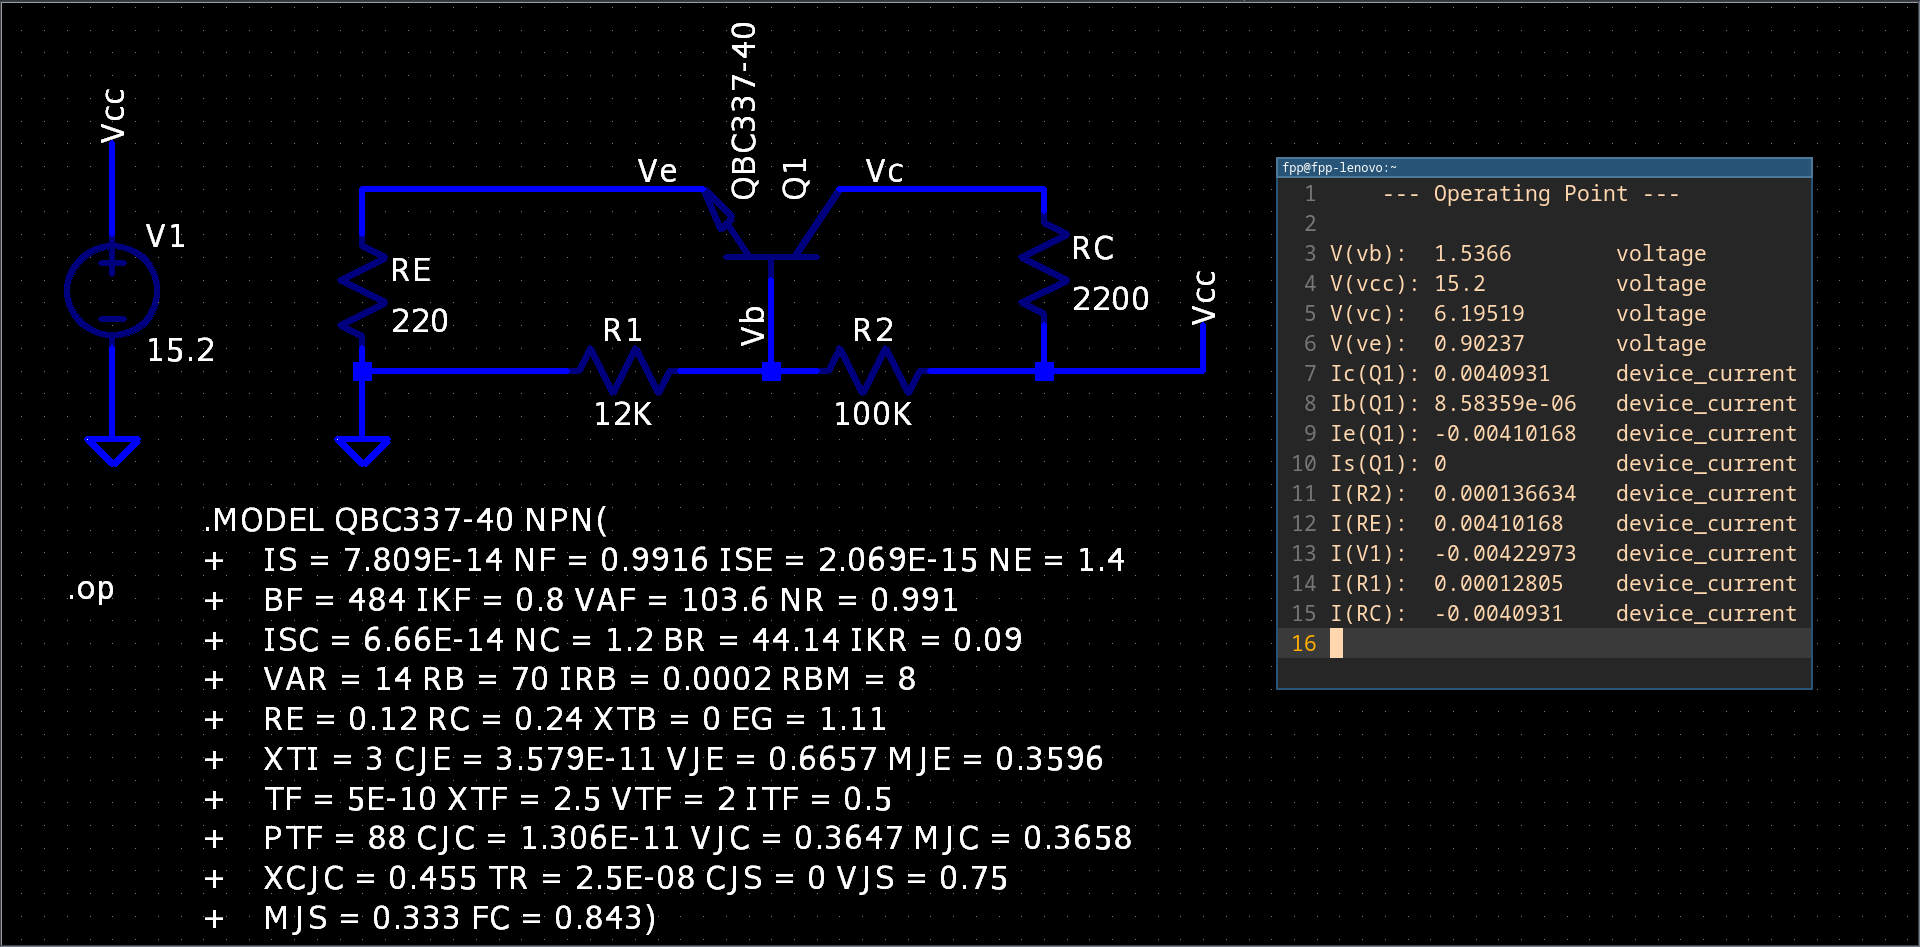
\includegraphics[width=.9\textwidth]{images/sim_normalizada.png}
    \caption{simulación en LTSpice de punto de operación (OP) con resistencias normalizadas.}
  \end{figure}
  \begin{equation*}
    4.07V \leq v_{CBQ} \leq 4.98V \quad \quad 3.7mA \leq i_{CQ} \leq 4.53mA
  \end{equation*}
\end{frame}

\subsection{Pequeña señal}
\begin{frame}[allowframebreaks]{Análisis de pequeña señal}
  \begin{figure}[ht!]
    \begin{minipage}[][\textheight][]{\textwidth}
      \centering
      \resizebox{\textwidth}{!}{
      \begin{tikzpicture}
        % Paths, nodes and wires:
        \draw (3.5, 1.25) to[american resistor, l_={$R_C$}] (3.5, -1.5);
        \draw (-3.5, -1.5) to[american resistor, l={$R_E$}] (-3.5, 1.25);
        \draw (5.5, 1.25) to[american resistor, l_={$R_L$}] (5.5, -1.5);
        \draw (-5.5, 1.25) to[sinusoidal voltage source, l_={$v_i$}] (-5.5, -1.5);
        \draw (-1.5, -1.5) to[american resistor, l={$h_{ib}$}] (-1.5, 1.25);
        \draw (1.5, 1.25) to[american current source, mirror, l_={$h_{fb} \cdot i_e$}] (1.5, -1.5);
        \draw (-5.5, -1.5) -- (7, -1.5);
        \node[ocirc] at (7, 1.25){};
        \node[ocirc] at (7, -1.5){};
        \draw (-5.5, 1.25) -- (-1.5, 1.25);
        \draw (1.5, 1.25) -- (7, 1.25);
        \node[shape=rectangle, draw, line width=0.5pt, dash pattern={on 2pt off 2pt}, minimum width=4.982cm, minimum height=4.482cm] at (-0, 0){};
        \node[ground] at (0, -1.5){};
        \draw[-latex] (-1.25, 0.75) |- (-1.75, 1.5);
        \draw[-latex] (-5.75, 0.75) -| (-5.75, 1.5) -- (-5.25, 1.5);
        \node[shape=rectangle, minimum width=0.715cm, minimum height=0.715cm] at (7, -0.25){} node[anchor=north west, align=left, text width=0.327cm, inner sep=6pt] at (6.625, 0.125){$v_o$};
        \node[shape=rectangle, minimum width=0.715cm, minimum height=0.715cm] at (-5.5, 1.875){} node[anchor=north west, align=left, text width=0.327cm, inner sep=6pt] at (-5.875, 2.25){$i_i$};
        \node[shape=rectangle, minimum width=0.715cm, minimum height=0.715cm] at (-1.5, 1.875){} node[anchor=north west, align=left, text width=0.327cm, inner sep=6pt] at (-1.875, 2.25){$i_e$};
        \draw[-latex] (-4.5, -2) -| (-4.5, -0.5) -- (-4, -0.5);
        \draw[-latex] (4.5, -2) |- (4, -0.5);
        \node[shape=rectangle, minimum width=0.715cm, minimum height=0.715cm] at (-4.5, -2.375){} node[anchor=north west, align=left, text width=0.327cm, inner sep=6pt] at (-4.875, -2){$Z_i$};
        \node[shape=rectangle, minimum width=0.715cm, minimum height=0.715cm] at (4.5, -2.375){} node[anchor=north west, align=left, text width=0.327cm, inner sep=6pt] at (4.125, -2){$Z_o$};
        \draw[-latex] (5.25, 1.5) -| (5.75, 0.75);
        \node[shape=rectangle, minimum width=0.715cm, minimum height=0.715cm] at (5.5, 1.875){} node[anchor=north west, align=left, text width=0.327cm, inner sep=6pt] at (5.125, 2.25){$i_l$};
        \node[shape=rectangle, minimum width=0.715cm, minimum height=0.715cm] at (1.5, 1.875){} node[anchor=north west, align=left, text width=0.327cm, inner sep=6pt] at (1.125, 2.25){$i_c$};
        \draw[-latex] (1.75, 1.5) -| (1.25, 1.5) -- (1.25, 0.75);
        \node[shape=rectangle, minimum width=0.715cm, minimum height=0.715cm] at (7, 0.875){} node[anchor=north west, align=left, text width=0.327cm, inner sep=6pt] at (6.625, 1.25){$+$};
        \node[shape=rectangle, minimum width=0.715cm, minimum height=0.715cm] at (7, -1.125){} node[anchor=north west, align=left, text width=0.327cm, inner sep=6pt] at (6.625, -0.75){$-$};
      \end{tikzpicture}
      }
      \caption{circuito equivalente para CA.}
    \end{minipage}
  \end{figure}

  \begin{figure}[!ht]
    \raggedright
    Podemos calcular las impedancias del amplificador:\\
    \centering
    \begin{minipage}[][\textheight][t]{0.45\textwidth}
      Usando (Ec. \ref{eq:hib}) y (Ec. \ref{eq:zi}):
      \begin{align*}
        h_{ib} &= \frac{25mV}{I_{CQ}}\\[6pt]
        Z_i &= R_E // h_{ib}\\[6pt]
        Z_i &= \frac{220\Omega \cdot \frac{25mV}{4.142mA}}{220\Omega + \frac{25mV}{4.142mA}}\\[6pt]
        Z_i &= 5.87\Omega
      \end{align*}
    \end{minipage}
    \hfill
    \begin{minipage}[][\textheight][t]{0.45\textwidth}
      Usando (Ec. \ref{eq:zo}):
      \begin{align*}
        Z_o &\approx R_C\\[6pt]
        Z_o &\approx 2K2\Omega
      \end{align*}
    \end{minipage}
  \end{figure}

  \begin{figure}[!ht]
    \raggedright
    Podemos calcular las ganancias del amplificador:\\
    \centering
    \begin{minipage}[t]{0.45\textwidth}
      Usando (Ec. \ref{eq:ai}):
      \small
      \begin{align*}
        A_i &= \frac{R_C}{R_C + R_L} \cdot \frac{R_E}{R_E + h_{ib}}\\[6pt]
        A_i &= \frac{2K2\Omega}{2K2\Omega + 2K2\Omega} \cdot \frac{220\Omega}{220\Omega + \frac{25mV}{4.142mA}}\\[6pt]
        A_i &= 0.486
      \end{align*}
    \end{minipage}
    \hfill
    \begin{minipage}[t]{0.45\textwidth}
      Usando (Ec. \ref{eq:av}):
      \small
      \begin{align*}
        A_v &= \frac{R_C // R_L}{h_{ib}}\\[6pt]
        A_v &= \frac{\frac{2K2\Omega \cdot 2K2\Omega}{2K2\Omega + 2K2\Omega}}{\frac{25mV}{4.142mA}}\\[6pt]
        A_v &= 182.248
      \end{align*}
    \end{minipage}
  \end{figure}

\end{frame}
